\documentclass[hidelinks]{article}

\usepackage[table,xcdraw]{xcolor}
\usepackage{graphicx}
\usepackage{lipsum}
\usepackage{tikz}
\usepackage{hyperref}
\usepackage{makeidx}
\usepackage{listings}
\usepackage{color}
\usepackage[letterpaper,margin=1in,footskip=0.5in]{geometry}
\usepackage{syntax}
\usepackage{booktabs}
\usepackage{longtable}
\usepackage{fancyhdr}
\usepackage{tcolorbox}

\newcommand{\revisionNumber}{DRAFT Revision 33 - 2023.05.16}
\fancypagestyle{revision}{
  \fancyhf{} % Clear header and footer fields
  \renewcommand{\headrulewidth}{0pt} % Remove header rule
  \fancyfoot[C]{Page \thepage\ | \revisionNumber} % Set the page number and revision number in the center of the footer
}
\pagestyle{revision}
	
\newcolumntype{b}{>{\hsize=0.2\hsize}X}
\newcolumntype{s}{X}

\makeindex

\title{\textbf{ABStract Language Specifcation}}
\date{\revisionNumber}
\author{\textbf{Author}\\John Dunlap\\\\\textbf{Acknowledgements}\\Daniel Pratt - Randall Fairman - Ryan Connolly}

\begin{document}
\pagenumbering{gobble}
\maketitle

\begin{center}
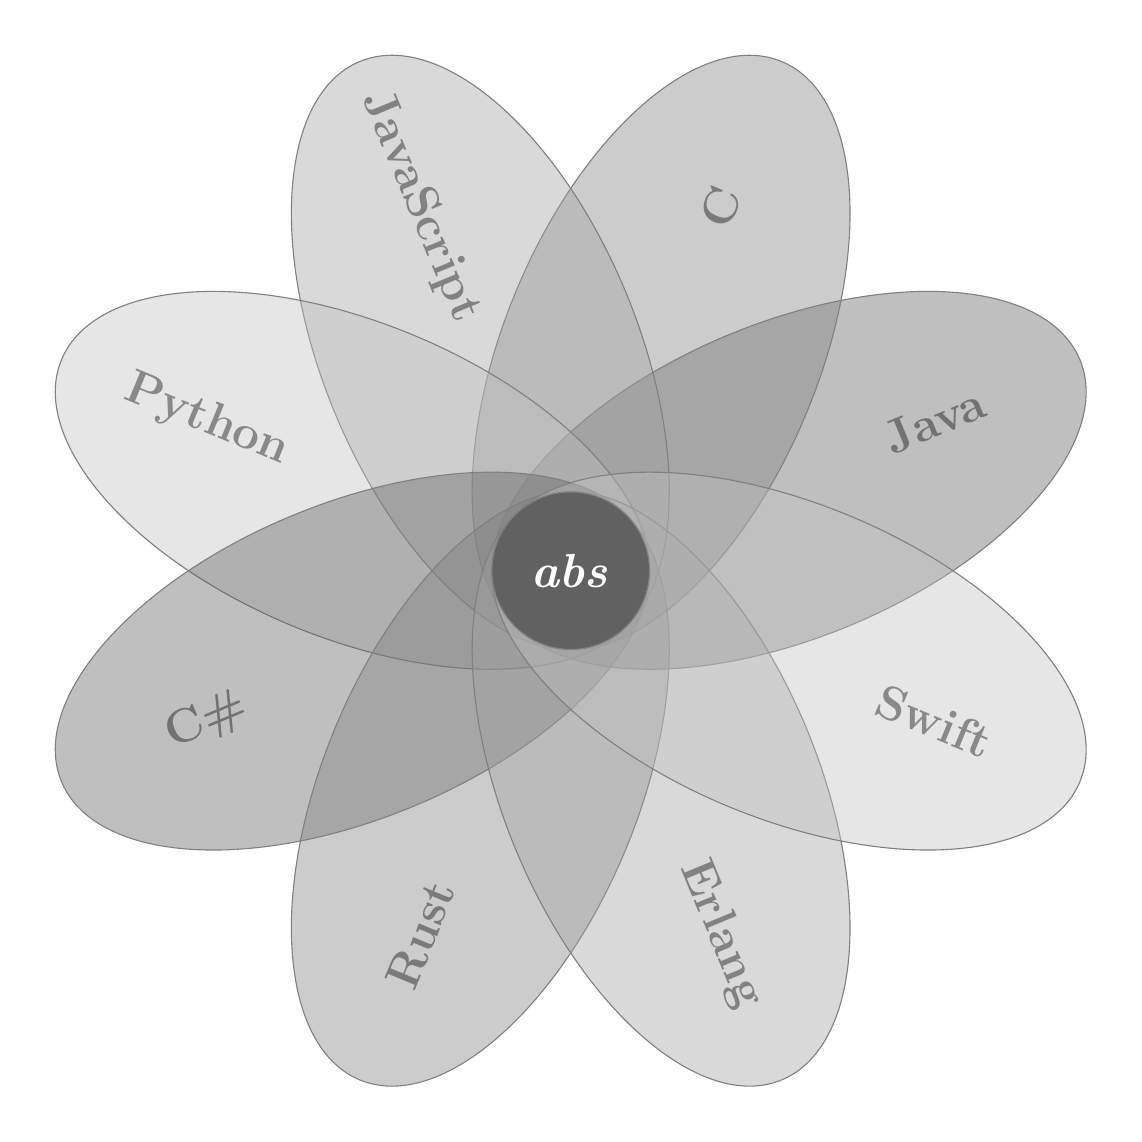
\begin{tikzpicture}
	\begin{scope} [fill opacity = .4]
	
	\definecolor{shade1}{RGB}{96,96,96}
	\definecolor{shade2}{RGB}{128,128,128}
	\definecolor{shade3}{RGB}{160,160,160}
	\definecolor{shade4}{RGB}{192,192,192}
	
	%% Draw ovals
    \draw[fill=shade1,    draw=gray, rotate=22.5]  (3,0) ellipse (4cm and 2cm);
    \draw[fill=shade2,    draw=gray, rotate=67.5]  (3,0) ellipse (4cm and 2cm);
    \draw[fill=shade3,    draw=gray, rotate=112.5] (3,0) ellipse (4cm and 2cm);
    \draw[fill=shade4,    draw=gray, rotate=157.5] (3,0) ellipse (4cm and 2cm);
    \draw[fill=shade1,    draw=gray, rotate=202.5] (3,0) ellipse (4cm and 2cm);
    \draw[fill=shade2,    draw=gray, rotate=247.5] (3,0) ellipse (4cm and 2cm);
    \draw[fill=shade3,    draw=gray, rotate=292.5] (3,0) ellipse (4cm and 2cm);
    \draw[fill=shade4,    draw=gray, rotate=337.5] (3,0) ellipse (4cm and 2cm);

    \draw[fill=black,    draw=gray]               (0,0) circle (1cm);

	%% Draw text on ovals
    \node[rotate=22.5]  at (4.62,1.91)   {\LARGE\textbf{Java}};
    \node[rotate=67.5]  at (1.91,4.62)   {\LARGE\textbf{C}};
    \node[rotate=337.5] at (-4.62,1.91)  {\LARGE\textbf{Python}};
    \node[rotate=292.5] at (1.91,-4.62)  {\LARGE\textbf{Erlang}};
    \node[rotate=292.5] at (-1.91,4.62)  {\LARGE\textbf{JavaScript}};
    \node[rotate=337.5] at (4.62,-1.91)  {\LARGE\textbf{Swift}};
    \node[rotate=67.5]  at (-1.91,-4.62) {\LARGE\textbf{Rust}};
    \node[rotate=22.5]  at (-4.62,-1.91) {\LARGE\textbf{C\#}};

	%% Draw center text
    \node[text=white, opacity=1] at (0,0) {\LARGE\textbf{\textit{abs}}};
    \end{scope}
\end{tikzpicture}
\end{center}

\newpage
\pagenumbering{arabic}
\tableofcontents{}
\newpage

\section{Introduction}
\paragraph{}The goal of the \textit{ABStract Programming Language}, hereafter referred to as \textit{abs}, is to cleanly share logic between wholly incompatible programming languages without introducing any dependencies beyond the logic itself.

\paragraph{}To achieve this goal, \textit{abs} has been designed as a transpiled programming language which enables unidirectional source-to-source transformation from \textit{abs} into other programming languages, hereafter referred to as targets. The initial list of supported targets is: Java, C\#, JavaScript, Erlang, Rust, C, Python, and Swift. By embracing dissimilar targets from day one, \textit{abs} benefits from a broader range of perspectives and ensures that its design is naturally bounded by commonalities between targets. This is why the \textit{abs} logo is a Venn diagram. 

\paragraph{}Commonalities between targets include, but are not necessarily restricted to: Variables, data types, functions, recursion, loops, if/else, arithmetic/logical operations, function call stack, and memory allocation.

\paragraph{}\textit{abs} supports three different kinds of functions: Native, pure, and impure. Native functions are \textit{abs} method contracts which define a name, return type, and argument list but which do not have a body. These methods are assumed to be implemented in the target language and available at runtime. Pure functions are functions which cannot call native functions either directly or indirectly. This is enforced by raising a compiler error if a pure function calls a function which is not also a pure function. Impure functions are functions which call functions of all types. Sharing state outside of method contracts is strictly forbidden and, consequently, \textit{abs} does not support global variables, singletons, static variables, or similar mechanisms. \textit{abs} does not guarantee the size of its numeric data types. At first glance, this may seem like inhibits portability but it is the position of this document that the opposite is true because this allows \textit{abs} to support different hardware platforms which have dissimilar CPU registers. This is similar to the approach taken by C which is, arguably, the most portable language ever created.

\paragraph{}However, there are also aspects of the \textit{abs} design with significantly differ from that of its supported targets. For example, \textit{abs} introduces support for multiple entry points, removes support IO of any kind, and prevents runtime errors at compile time. Multiple entry points are necessary because native code, written in a target language, must be able to directly call \textit{abs} functions. Support for IO is not provided because \textit{abs} is dependent on the target to provide this functionality through native methods.  


\subsection{Why Another Language?}
\paragraph{}
The world is full of weird and wonderful programming languages which aim to solve problems in every way you can imagine and likely a few ways you can't. At the time this was written, there were 694 programming languages listed on \href{https://en.wikipedia.org/wiki/List_of_programming_languages}{{\color{blue}Wikipedia}}\footnote{\url{https://en.wikipedia.org/wiki/List_of_programming_languages}.}. Every programming language has its pros and cons but, at this point, it's very unusual to encounter a problem which cannot be solved with at least one of them. The enescapable question which must be answered by every language designer is this: Why does a world with so many programming languages need another one? While it is certainly true that there are very few tasks, if any, which cannot be solved with an existing programming language, it is important to remember that this has always been the case. For example, there are no solvable problems which cannot be solved with assembly language and yet more than 600 programming languages have been created since assembly language was created. Just because it's possible to solve a problem with a particular language does not necessarly mean that it's the best tool for the job, even if it's the only available tool. Programming languages are created for a variety of reasons including expressiveness, domain specific needs, performance, parallelism, simplification, compatibility, etc. The need driving the creation of \textit{abs} is broad compatibility. Certainly, you could write the same function multiple times, once for each of your deployment environments but it would be more efficient and preferable to write that function once and compile it separately for each of your deployment environments.

\subsection{Design Descisions}
\subsubsection{Memory Management}
\paragraph{}Within the initial list of targets, there are four distinct approaches to memory management: 
\begin{longtable}{ |p{4cm}|p{11cm}|  }
\hline
\textbf{Approach} & \textbf{Targets} \\
\hline
Garbage collected heap memory & Java, C\#, Erlang, Swift, Python, JavaScript\\
&\\
\hline
Manually managed heap memory & C\\
&\\
\hline
Smart pointer managed heap memory & Rust\\
&\\
\hline
Automatically managed stack memory & All\\ 
&\\
\hline
\end{longtable}
\paragraph{}Automatic memory management is a fundamental design goal of \textit{abs}. Unfortunately, not all targets support it. C defers heap management to the programmer, Rust requires the explicit use of smart pointers, and other targets rely on garbage collectors to manage the heap. This inconsistency forces \textit{abs} to include memory management in its design such that it it is possible to support targets which do not have a garbage collector.

\paragraph{}It is not feasible to implement a portable garbage collector for targets which do not already have one. The simplest solution to this problem is to add compile time constraints which which have no affect in targets other than C while allowing \textit{abs} to implement a stack managed heap when targeting C.

\subsubsection{Types}
\subsubsection{Error Handling}
\subsubsection{Null References}
\paragraph{}To null or not to null? That is the question. In 1965, \href{https://en.wikipedia.org/wiki/Tony_Hoare}{{\color{blue}Tony Hoare}}\footnote{\url{https://en.wikipedia.org/wiki/Tony_Hoare}.} changed computer science forever by introducing null references in \textit{ALGOL W}. In 2009, having observed his invention for 44 years, he had this to say:
\paragraph{}\textit{"I call it my billion-dollar mistake. It was the invention of the null reference in 1965. At that time, I was designing the first comprehensive type system for references in an object oriented language (ALGOL W). My goal was to ensure that all use of references should be absolutely safe, with checking performed automatically by the compiler. But I couldn't resist the temptation to put in a null reference, simply because it was so easy to implement. This has led to innumerable errors, vulnerabilities, and system crashes, which have probably caused a billion dollars of pain and damage in the last forty years." - Tony Hoare}

\paragraph{}Did Mr. Hoare fail to solve the problem of unsafe references? Null references are clearly unsafe.

\textbf{TODO: This doesn't read well and comes across as being very clumsily written}
Let's take a step back and look at what Mr. Hoare's goal was when he invented null references. He said, \textit{"My goal was to ensure that all use of references should be absolutely safe, with checking performed automatically by the compiler."} If unsafe references existed prior to null references then it seems reasonable to infer that reference errors were the underlying problem he was attempting to solve. 

It seems as if the problems Mr. Hoare attributes to null references, in the quote above, are the very similar to the problems he originally set out to solve. 

Is the answer simply that Mr. Hoare failed to solve the problem of unsafe references? Not exactly. Reference errors existed both before and after the invention of null references so, in that sense, you could say that he failed. However, in fairness to Mr. Hoare, he succeeded in reducing the number of invalid references from many to one. This is no small feat and represents a major step forward in the field of computer computer science because it replaces complicated address range checks with a single equality comparison. This equality comparison allows higher level languages to safely report reference errors, gracefully fail, and even recover from reference errors without crashing the entire program. Unfortunately, this has led to the unfair perception that null is the root of the problem and it isn't. It doesn't matter if the address of an invalid reference is zero or some other value. If a program attempts to dereference an invalid reference, there will be an error. Period. If a compiler allows a program to dereference an invalid reference be it a null reference or not then the fault lies with the compiler. When these errors occur, null isn't an antagonist; It is a messenger.

\paragraph{Should \textit{abs} support null?}From a pragmatic perspective, the answer must be: Yes. Due to \textit{abs} being a transpiled language, many of its compilation targets will support null and refusing to support null would complicate the interaction between native and non-native methods. Null references exist; That is a fact. Whether or not they \textit{should} exist isn't relevant. What happens if \textit{abs} does not support null and a native method returns null or passes null into an \textit{abs} entry point? It's inconcievable that this would never happen in practice and, consequently, it must be accounted for in the design of the language. There are other ways to approach the problem but it is the position of this document that supporting null references is, by far, the simplest.

\subsection{Why have cross platform languages failed in the past?}
\paragraph{}\textbf{TODO: Define what is meant by "failed". What would success look like for a cross platform language? Did Java really fail? It's one of the most popular languages ever created.} Most modern programming languages are capable of implementing any other programming language. However, just because language A can be used to implement language B doesn't necessarily mean that the resulting implementation of language B will perform well enough to be useful outside an academic setting.
\paragraph{}The Java Programming Language\footnote{\url{https://en.wikipedia.org/wiki/Java_(programming_language)}} boasts \textit{"Write once. Run anywhere"}. While this was mostly true when Java was originally created, it has become less and less true over time. The problem is that Java programs can only be run on platforms which are supported by the JVM\footnote{\url{https://en.wikipedia.org/wiki/Java_virtual_machine}} and the number of available platforms, in combination with the increasing complexity of the JVM, has made it very difficult for Java to support all of them. To make matters worse, even if a platform is supported by the JVM, the platform may prohibit the installation of the JVM, may provide an API or SDK which is not written in Java, or the JVM may be too resource intensive to be viable on the target platform. At this point, no language runtime has achieved the level of dominance necessary to be available on every platform, it seems unlikely that any languge runtime will achieve this level of dominance, and even if a language runtime were to achieve this level of dominance, it is unlikely that it could maintain this level of dominance indefinitely. Given the apparent impossibility of this dilemma, \textit{abs} has chosen to abandon the concept of a language runtime entirely. Every platform which currently exists, or which is likely to exist, will support at least one programming language so there is no need to provide a language runtime in the first place. It is, therefore, the goal of the \textit{abs} compiler to leverage whatever language, API, or SDK is available on the target platform. This goal has lead to the ideal: \textit{"Write once. Compile anywhere."}
\textbf{TODO: Expand on the idea that Java's downfall was too many runtime dependencies.}
\subsection{Why aren't cross platform languages the norm?}
\textbf{TODO}Cross platform languages are hard. Different languages have different capabilities, strengths, and weaknesses. Too many features; Every supported feature complicates adding support for new platforms. Designing a language which is functionally divergent from the platforms on which it needs to run. Too much complexity. Failure to constrain language semantics to the overlapping capabilities of the platforms which must be supported. Similar or identical problems are solved in different ways on different platforms. Attempting to solve the same problem in a portable way may 
\subsection{Problems}
The following are problems which are not, either in whole or in part, solved by existing languages.
\subsubsection{Multiple Platforms}\paragraph{}One of the principle challenges in modern software development is supporting the ever increasing number of platforms and smart devices. Many of these devices, despite supporting similar use cases, technically have very little in common with one another. These devices have different form factors, different operating systems, different hardware, different language support, different libraries, and different distrubution mechanisms. Consequently, supporting multiple devices is more expensive than supporting a single device and every additional supported device increases costs and extends deadlines.
\subsubsection{Limited Reusability}\paragraph{}The word "abstract" can mean different things. In the context of this document, it is a programming language. In conversation, it can mean something is difficult to understand or it can refer to an idea. In the context of an object oriented programming language, it refers to classes which are intended to address the overlap between two or more similar problems. Code which is useful in multiple problems is included and code which is only useful for a single problem is excluded. This allows an unknown number of similar problems to be partially solved while fully solving a single problem. This is a valuable capability which simplifies the creation of reusable software. However, it does have limitations. Although many languages support the concept of an abstract class, in one form or another, an abstract class in languge A is, generally speaking, wholly incompatible with language B. Consequently, an abstract class isn't truly abstract because it must be written separately in each language which requires it. This inability to share abstract classes between languages and platforms is one of the reasons that supporting two or more platforms more expensive than supporting a single platform.
\textbf{TODO: Limited reusability is a problem which applies to more than just abstract classes. For example, a function written in language A cannot be reused in language B}
\subsubsection{Premature Obsolescence}\paragraph{}Software applications degrade over time, for a variety of reasons, and, while some degrade more quickly than others, in the absence of extraordinary intervention, they all, eventually, reach the end of their useful service life. This degredation is, unfortunately, unavoidable because it is caused by the very technical implementation details which make the application functional. Over time, technical implementation details become increasingly intertwined with business logic and, past a certain point, it becomes impractical to separate them. Many software applications continue like this until it becomes necessary to retire their underlying technology which, in turn, forces the organization to retire the application as well. This is unfortunate because organizations invest decades of time, money, knowledge, and effort into building software applications which still have value at the point that they must be retired. Replacing these software applications is difficult, time consuming, and expensive.
\subsubsection{Conflict Of Interest}\paragraph{}The interests of corporations, which provide free software development tooling, are not always aligned with the interests of those who use their tooling. If a corporation spends a large amount of money developing tools which they subsequently give away for free, there's very rarely an altruistic explanation. Common explanations include, but are not limited to, a corporation wants you to use their hardware, their operating system, or their platform and, consequently, makes it as easy as possible for you to do so. Whatever their reason happens to be, the use of their tools is usually a mutually beneficial relationship. However, it should be self evident that a corporation which offers free tools for building applications on their own platform cannot be relied upon also provide free tools for building applications on their competitors platforms. They may do it, under some circumstances, particularly if they are not the market leader, but they may discontinue support for their competitor's platforms, at any time and without warning, if it becomes too expensive or if they achieve market dominance. It is in the best interest of a corporation for application X to exclusively support their platform. By contrast, it is in the best interest of the consumer to for application X to support as many platforms as possible because this gives them the freedom to choose which platform works best for them. 
\subsubsection{Monolingual applications are expensive}\paragraph{}
\textbf{TODO: Fill this out}
\subsection{Solution}
It is the position of this document that there can be no solution to the problems outlined above except the creation of a new programming language.
\\
\subsection{Philosophy}
The design of the \textit{abs} language is guided by the principles found below. Some of these principles may be familiar to the discerning eye. This is because principles deemed to have value, in the context of \textit{abs}, have been adopted from other projects.
\begin{itemize}
  \item \textbf{Do one thing and do it well:} Don't try to be all things to all people. The goal is portable logic. Nothing more. Nothing less.
  \item \textbf{Compilation errors are better than runtime errors:} Errors encountered by a developer are better than errors encountered by a user. Minimize runtime errors by maximizing compilation errors.
  \item \textbf{Portability is more valuable than performance:} Without portability, there is no reason for \textit{abs} to exist. Performance matters but portability should never be sacrificed in pursuit of it.
  \item \textbf{Pragmatism in all things:} Ideas are only useful insofar as they help us solve the problem at hand. If a good idea detracts from our ability to solve a problem then that idea must inform our solution rather than embody it.
  \item \textbf{Simple is better than complex:} Portability increases as complexity decreases. \textit{The best part is no part} - Elon Musk
  \item \textbf{Explicit is better than implicit:} Make intentions and behaviors clear, rather than relying on implicit or obscure mechanisms.
  \item \textbf{Readability counts:} \textit{Any fool can write code that a computer can understand. Good programmers write code that humans can understand} - Martin Fowler
\end{itemize}
\subsection{Security Considerations}
\subsubsection{Native Code Injection}
Native code injection attacks are very similar to SQL injection attacks. When accepting user created code, string concatenaction is extremely dangerous because the user could attempt to escape the compiler's sandbox by embedding native code in a string constant, which would be ignored by \textit{abs} but not by the compiler of the native language, with the goal of accessing native resources which would not otherwise be available. One possible solution to this problem would be to store all string constants in a text file which gets automatically loaded at runtime by the code which is emitted by the compiler.
\subsubsection{Denial Of Service}
If abs code is accepted from users then, in the absence of some kind of timeout, code which loops or iterates infinitely could be used to execute a denial of service attack.
\subsubsection{Types}
\paragraph{}The principal hurdle of building a portable type system is ensuring consistency and compatibility across multiple target languages. Transpilation involves converting code from one language to another, each with its own type system and semantic rules. Mapping types accurately between the source language and target languages can be complex, as different languages may have different type representations, behavior, and limitations. Maintaining semantic integrity and ensuring that the type system behaves consistently across targets requires careful consideration and meticulous design. Another challenge is dealing with language-specific features and constructs that may not have direct equivalents in all target languages. Balancing the expressiveness of the type system while accommodating the constraints and limitations of the target languages is crucial. Furthermore, error reporting and debugging can be challenging when dealing with type-related issues in a transpiled language, as the error messages need to be meaningful and provide insights that align with the target language's conventions and error reporting mechanisms. Overall, creating a portable type system in a transpiled language necessitates a deep understanding of both the source and target languages, as well as careful planning and implementation to address the inherent challenges of cross-language compatibility and semantic consistency.
\subsubsection{Boolean truth}
\begin{tcolorbox}[colback=gray!20, colframe=gray!50!black, arc=4mm]
TODO: Describe the pros and cons of "truthiness" vs actual boolean types.
\end{tcolorbox}

\subsubsection{Error handling}
\paragraph{}Errors are inevitable and, consequently, it is necessary to both detect and react to them. 
\\
How do we implement exceptions in a language which doesn't natively support them(Like C)?
\\
This must be taken into account in the architecture of every programming language. The are many ways to approach this problem but two popular approaches are returning error codes from functions in the case of an error or throwing an exception and rolling up the call stack until the exception is handled. In this section we will be exploring the pros and cons of the two approaches.

\begin{itemize}
\item Method calls can fail for multiple reasons.
\item Calling code may need to know what those reasons are.
\item Failing early is not necessarily better.
\item In some circumstances, it may be preferable for execution to continue after an error.
\item In some circumstances, it may be preferable for execution to halt after an error.
\end{itemize}
\subsection{Versioning}
\textbf{TODO: }It must possible to lexicographically compare versions with string operators to determine which version is newer. Older versions should always be lexicographically lesser than newer versions.
\newpage
\section{Specification}
\subsection{Definition Of Terms}
\subsubsection{Base Language}
Any language which is supported as an \textit{abs} compilation target.
\subsubsection{Pure function}
A pure function is any function which does not either directly or indirectly invoke a native method. This results in functions which do not have external dependencies.
\subsubsection{Impure function}
An impure function is not declared as native or pure and is able to call all types of functions.
\subsubsection{Native function}
Native functions do not have a body because they are assumed to have been implemented in the target language and to be available at runtime.
\subsection{Literals}
\subsubsection{Number Literal}
Number literals are comprised of the characters 0 through 9 and may not contain a decimal point. If a number literal is terminated with the letter L, case sensitive, then it is of type Long. Ohterwise, it is of type Integer. Number literals may use underscores as separators to make large numbers easier to read. Number literals which begin with 0x are hexidecimal. In hexadeciam numbers, underscores are not permitted until after the 0x. Leading zeros are ignored in all bases. Number literals may be prefixed with a minus sign or a plus sign to indicate the sign of the literal.

\subsubsection{Decimal Literal}
\textbf{TODO:} Decimal literals must contain a decimal point.

\subsubsection{String Literal}
String literals may contain any UTF-8 character. Double quote characters must be escaped with a backslash to avoid prematurely terminating the String literal. String literals may also contain interpolated variables. An interpolated variable must begin with a dollar sign. Dollar signs which are a part of the string literal must be escaped with a backslash character. If necessary, after the dollar sign, the name of the interpolated variable may be enclosed in curly braces to prevent characters from the string literal being included in the interpolated variable name.

\subsubsection{Boolean Literal}
Legal values are \textbf{true} and \textbf{false}.

\subsubsection{Null Literal}
\textbf{null} is the only legal value.

\subsubsection{Paradigm Literal}
Legal values are \textbf{oop}, \textbf{procedural}, and \textbf{functional}.
\subsection{Reserved Words}
It is illegal for any namespace, function, or variable name to coincide with a reserved word. Reserved words are case insenstive.
\begin{longtable}{ |p{4cm}|p{11cm}|  }
\hline
\textbf{Word} & \textbf{Description} \\
\hline
\textbf{coalesce} & Built-in method which accepts two or more parameters and returns its first non-null parameter or null if all parameters evaluate to null. The first parameter must be nullable. The last parameter may be nullable or non-nullable. If there are intermediate parameters, all of them must be nullable. Parameters are evaluated from left to right. All parameters must be the same type. The nullability of the return is inherited from the last parameter. It is illegal for any of the parameters to be a null literal.\\
&\\
\textbf{nullable} & Variable modifier which permits null assignment. In the absence of this modifier, the compiler will emit an error when an assignment operation may result in null assignment. This modifier may also be used on the function return type or function parameters. \textbf{TODO: This should be revisited it would be simpler to follow the .NET ? approach to determining nullability} \\
&\\
\textbf{pure} & Namespace modifier which prevents methods within the namespace from interacting with other namespaces which haven't also been declared as pure. This modifier is mutually exclusive with the native modifier. Pure namespaces may not interact with impure namespaces but impure namespaces may interact with pure namespaces. This increases the portability of pure namespaces because the \textit{abs} compiler is able to verify, at compile time, that pure namespaces do not have any native dependencies.\\
&\\
\textbf{native} & Namespace modifier which indicates that methods declared within the namespace must be implemented separately in each target language. Method declarations within a native namespace should be terminated with a semicolon as it is illegal for them to have a body. This modifier is mutually exclusive with the pure modifier. It is illegal for a native method to be declared as returning a value which is non-nullable or a type which, either directly or indirectly, containes one or more properties which are non-nullable because the return value of a native method cannot be known until run time and, therefore, cannot be checked for null at compile time.\\
&\\
\textbf{entry} & Method modifier which declares a method as an entry point into an \textit{abs} program. This is necessary because compile time null checking is not possible if a native method, which isn't written in \textit{abs}, can invoke any \textit{abs} method at any time because the provided arguments might be null at run time even if the method in question expects non-nullable parameters. Consequently, methods declared as an entry point may not directly or indirectly accept parameters which have not been declared as nullable. This forces explicit null checking to be performed prior to invoking functions which do not accept nullable parameters. Additionally, the \textit{abs} compiler may obfuscate functions in its output which have not been declared as an entry point to discourage their use in native functions as doing so would create the possibility of a null pointer exception. This modifier may be used within a pure namespace. It is an error to use this modifier within a native namespace. \\
&\\
\textbf{final} & Variable modifier which indicates that the value of the variable cannot be changed. \\
&\\
\textbf{in} & Operator which evaluates to true if the value on its left side exists in the collection on its right side and evaluates to false otherwise. It is illegal for the value on its left side to be null. \\
&\\
\textbf{void} & Function modifier which indicates that a function does not return a value. \\
&\\
\textbf{return} & Operator which immediately halts execution of the function in which it is invoked. This operator must be invoked without an argument if the function was declared with a void return type and must be invoked with a single argument otherwise. If invoked with a single argument, the argument will be returned to the invoking function. It is an error for the type or nullability of the argument to differ from that of the return type which was declared in the method signature. \\
& \\
\hline
\end{longtable}

\begin{tabular}{llllllllll}
synchronized & null & not null & package & \\
assert & class & enum & use & this & finally & \\
final & abstract & double & super & transient & public & private & protected & \\
for & do & true & false & while & \\
break & byte & case & virtual & switch & continue & throws & throw & \\
new & catch & if & implements & try & else & oop & \\
functional & procedural & set & get & goto & integer & struct & \\
string & float & boolean & thread & base & default & alias & narrow \\
\end{tabular}
\subsection{Grammar}
\subsubsection{Object Oriented}
\subsubsection{Procedural}
\begin{grammar}

<statement> ::= <ident> `=' <expr> 
\alt `for' <ident> `=' <expr> `to' <expr> `do' <statement> 
\alt `{' <stat-list> `}' 
\alt <empty> 

<stat-list> ::= <statement> `;' <stat-list> | <statement> 

\end{grammar}
\paragraph{Increase the two lengths}
\setlength{\grammarparsep}{20pt plus 1pt minus 1pt} % increase separation between rules
\setlength{\grammarindent}{12em} % increase separation between LHS/RHS 

\begin{grammar}

<statement> ::= <ident> `=' <expr> 
\alt `for' <ident> `=' <expr> `to' <expr> `do' <statement> 
\alt `{' <stat-list> `}' 
\alt <empty> 

<stat-list> ::= <statement> `;' <stat-list> | <statement> 

\begin{syntdiag}<ident> ‘(’
	\begin{rep} \begin{stack} \\
		<type> \begin{stack} \\ <ident> \end{stack}
	\end{stack} \\ ‘,’ \end{rep}
\begin{stack} \\ ‘...’  \end{stack} ‘)’
\end{syntdiag}

\end{grammar}
\begin{enumerate}
\item \textbf{allow-functions-outside-class} - In languages which do not natively support OOP or where OOP is optional, it can be useful to declare functions outside class definitions. This feature could also be useful when transpiling other languages to \textit{abs}. This feature is disabled by default but can be enabled by passing an option to the compiler. 
\item \textbf{allow-variables-outside-class} - In languages which do not natively support OOP or where OOP is optional, it can be useful to declare variables outside class definitions. This feature could also be useful when transpiling other languages to \textit{abs}. This feature is disabled by default but can be enabled by passing an option to the compiler. 
\end{enumerate}
\subsection{Accessors}
\textit{abs} uses the same syntax to access attributes whether they have accessor methods or not. This allows accessor methods to be added or removed at a later date without breaking compatibility with code outside of the class definition.
\subsection{Operators}
\begin{longtable}{ |p{4cm}|p{3cm}|p{8cm}|  }
\hline
\textbf{Operator} & \textbf{Type} & \textbf{Description} \\
\hline
\textbf{+}                         & Math    & Numeric addition operator. Used for both integer and float types                   \\
\textbf{+=}                        & Math    & Numeric addition-assignment operator. Used for both integer and float types \\
\textbf{-}                         & Math    & Numeric subtraction operator. Used for both integer and float types                   \\
\textbf{-=}                        & Math    & Numeric subtraction-assignment operator. Used for both integer and float types \\
\textbf{\texttt{*}}                & Math    & Numeric multipaction operator. Used for both integer and float types                   \\
\textbf{\texttt{*}=}               & Math    & Numeric multipaction-assignment operator. Used for both integer and float types \\
\textbf{/}                         & Math    & Numeric division operator. Used for both integer and float types                   \\
\textbf{/=}                        & Math    & Numeric division-assignment operator. Used for both integer and float types \\
\textbf{\%}                         & Math    & Numeric modulus operator. Used for both integer and float types                   \\
\textbf{\%=}                        & Math    & Numeric modulus-assignment operator. Used for both integer and float types \\
\textbf{++}                         & Math    & Numeric increment operator. Used for both integer and float types                   \\
\textbf{--}                         & Math    & Numeric decrement operator. Used for both integer and float types                   \\
\textbf{==}                        & Logical & Logical equality operator. This operator will evaluate to true if the expression on both sides evaluate to the same value. Otherwise, this operator will evaluate to false. This is used for integer, float, and string types.                 \\
\textbf{\textless}                 & Logical & Logical less-than operator. This is used for integer, float, and string types.                   \\
\textbf{\textgreater}              & Logical & Logical greater-than operator. This is used for integer, float, and string types                   \\
\textbf{\textless=}                & Logical & Logical less-than-or-equal operator. This is used for integer, float, and string types                   \\
\textbf{\textgreater=}             & Logical & Logical greater-than-or-equal operator. This is used for integer, float, and string typesr                   \\
\textbf{!}                         & Logical & Logical NOT operator. This is a unary operator which evaluates to the opposite of what its expression                   \\
\textbf{!=}                        & Logical & Logical not-equal operator. This is a binary operator which evaluates to the opposite of what its argument evaluates to. This is used for integer, float, and string types                   \\
\textbf{\&\&}                      & Logical & Logical AND operator                   \\
\textbf{\textbar\textbar}          & Logical & Logical OR operator                   \\
\textbf{in}                        & Logical    & Binary operator which evaluates to true if the value on its left exists within the collection on its right and evaluates to false otherwise \\
\textbf{and}                        & Bitwise & Bitwise AND operator                   \\
\textbf{and=}                       & Bitwise & Bitwise AND-assignment operator        \\
\textbf{nand}                        & Bitwise & Bitwise NAND operator                   \\
\textbf{nand=}                       & Bitwise & Bitwise NAND-assignment operator        \\
\textbf{or}                  & Bitwise & Bitwise OR operator                    \\
\textbf{or=}                 & Bitwise & Bitwise OR-assignment operator         \\
\textbf{xor}                      & Bitwise & Bitwise XOR operator                   \\
\textbf{xor=}                     & Bitwise & Bitwise XOR-assignment operator        \\
\textbf{xnor}                      & Bitwise & Bitwise XNOR operator                   \\
\textbf{xnor=}                     & Bitwise & Bitwise XNOR-assignment operator        \\
\textbf{nor}                      & Bitwise & Bitwise NOR operator                   \\
\textbf{nor=}                      & Bitwise & Bitwise NOR-assignment operator                   \\
\textbf{comp}                      & Bitwise & Bitwise complement operator            \\
\textbf{comp=}                     & Bitwise & Bitwise complement-assignment operator \\
\textbf{lshift}        & Bitwise & left-shift operator            \\
\textbf{lshift=}       & Bitwise & left-shift-assignment operator \\
\textbf{rshift}  & Bitwise & right-shift operator           \\
\textbf{rshift=}       & Bitwise & right-shift-assignment operator \\
\textbf{?:}                        & Misc    & Ternary operator \\
\textbf{=}                         & Misc    & The assignment operator assigns the computed value on the its right side to the variable on its left side \\
\textbf{isa}                & Misc    & This operator evaluates to boolean true if the expression on its left is polymorphically and instance of the expression on its right. Otherwise, it evaluates to boolean false \\
\textbf{new}                       & Misc    & This operator creates new instances of a class \\
\textbf{throw}                     & Misc    & This operator throws a new exception \\
\textbf{\textbar}      & Misc    & The pipe operator allows the output of one method to be chained into the input of another method, even if those methods do not belong to the same class. The method on the right must only accept a single parameter and the type of that parameter must match the return type of the function on the left.
\\
\hline
\end{longtable}

\subsection{Types}
\subsubsection{Supported}
\begin{enumerate}
\item Integer(i32)
\item Long(int64)
\item Float(f32) - IEEE Standard 754 Single Precision
\item Double(f64) - IEEE Standard 754 Double Precision
\item Fixed - Fixed point precision
\item number\textless{}M\textgreater{} - M is the required digits to the right of the decimal point
\item number\textless{}N,M\textgreater{} - N is the number of required digits to the left of the decimal point and M is the required digits to the right of the decimal point
\item String
\item Byte - This is the only data type which is supported for binary operations.
\item Date - Date only. No timestamp.
\item DateTime - Date and timestamp.
\item Boolean - Used for all boolean operations.
\item Array\textless{T}\textgreater
\item Map\textless{K,V}\textgreater
\item User defined 2 dimensional data structures(classes).
\end{enumerate}
\subsubsection{Mapping}
ABS types will be translated to target languages as follows:\\
\begin{tabular}{llllllll}
                  & \textbf{Perl} & \textbf{Java}                       & \textbf{PHP} & \textbf{JS} & \textbf{C++} \\
\textbf{Integer}  & scalar        & Integer                             & dynamic      & dynamic     & int             \\
\textbf{Long}     & scalar        & Long                                & dynamic      & dynamic     & long             \\
\textbf{Float}    & scalar        & Float                               & dynamic      & dynamic     & float             \\
\textbf{Double}   & scalar        & Double                              & dynamic      & dynamic     & double             \\
\textbf{String}   & scalar        & String                              & dynamic      & dynamic     & std::stringstream          \\
\textbf{Byte}     & scalar        & Byte                                & dynamic      & dynamic      & unsigned char             \\
\textbf{Date}     & ???        & Date                                & dynamic      & dynamic     & ???             \\
\textbf{DateTime} & ???        & Date                                & dynamic      & dynamic     & ???             \\
\textbf{Boolean}  & scalar        & Boolean                             & dynamic      & dynamic     & bool             \\
\textbf{Array}    & arrayref      & ArrayList\textless{}T\textgreater{} & array        & array       & std::vector             \\
\textbf{Map}      & hashref       & HashMap\textless{}K,V\textgreater{} & array        & object     & std::map            
\end{tabular}
\\\\\\
\textbf{For the time being, the following languages have been omitted from this list:}
\begin{enumerate}
\item \textbf{C} - Because it does not support OOP and because it does not support throw/catch exception semantics.
\item \textbf{Elixir} - Because it does not support OOP.
\end{enumerate}

\newpage
\subsubsection{Narrowing}
Narrow types like \textbf{uint8} will be be masked when necessary to provide "proper" narrow types on platforms which don't support them. Masking is necessary in the following situations:
\begin{enumerate}
\item When passing the value to an arbitrary function which is not known to tolerate "trash upper bits".
\item When storing the value to a storage location that does not automatically truncate the value.
\item Before specific operations, namely: shift right, divide, remainder, compare, conversion to a wider or floating point type
\end{enumerate}
Most operations, namely AND, OR, XOR, NOT, shift-left, addition/subtraction/negation, multiplication and conversion to a narrower type, are not affected by "trash upper bits". The trash stays safely contained in those upper bits, which will be ignored in the end.

JavaScript and its floats are a bit trickier, because floats can throw away the bottom bits, which is bad. In fact, just multiplying two 32bit integers is non-trivial in JavaScript.
\newline\noindent
\textbf{TODO: Reword this section because it is copied from the internet}
\subsection{Command Line Interface}
The command line interface, hereafter referred to as the \textit{cli}, houses all of the native code necessary for interacting with the \textit{abs} compiler. It is important to differentiate between the \textit{abs} \textit{cli} and the \textit{abs} compiler because the compiler is written in \textit{abs} and the \textit{cli} is not. This is a direct consequence of the \textit{abs} language specification, which prohibits direct acccess to native functionality. While there is only one \textit{abs} compiler, there could, theoretically, be as many as one \textit{cli} per supported platform. Available \textit{cli} functionality includes, but is not limited to, the ability to compile, refactor, reformat, and query \textit{abs} code. 

\paragraph{target directory} All files created by the \textit{abs} compiler will be placed in a directory called \textbf{target} within the project root directory. This makes it easy to to manually clean up after the compiler.
\section{Road Map}
\subsection{Milestones}
	\begin{itemize}
		\item Build a lexer in Java
		\item Build a parser in Java
		\item Build an interpreter. This interpreter will be used to execute the initial compilation targets, which will be written in \textit{abs} rather than the host language.
		\item Compile to a single target
		\item Compile to multiple targets
		\item Rewrite the compiler in \textit{abs}
		\item Self compilation
	\end{itemize}
\subsection{Command Line utility: absc}
The \textit{absc}(ABS Compiler) utility will be a combination of various native stubs and a C++ version of the abs compiler which can be installed through the package managers of popular linux distributions.
\subsection{IDE Plugins}
IDE plugins are central to the adoption strategy of the platform as a whole. The compiler itself should be embedded into IDE plugins for all popular IDEs. These would include but not be limited to:
	\begin{itemize}
		\item Jetbrains
		\item Eclipse
		\item Netbeans
		\item Code Blocks
		\item CodeMirror
		\item Ace
		\item VSCode
		\item Monaco
	\end{itemize}
\subsection{Compilation Targets}
These are the language targets which will be implemented first.
	\begin{itemize}
		\item Haxe - Indirectly provides other targets including JavaScript and PHP
		\item Perl - Not provided by Haxe
		\item Elixir - Not provided by Haxe
	\end{itemize}
Additionally, compilation targets for the following languages are planned for the future.
	\begin{itemize}
		\item PHP
		\item Javascript
		\item Java
		\item C\#
		\item C++
		\item C
		\item Rust
		\item Python
		\item Perl
		\item Lua
		\item XML Schema(This would only export data structures, not behavior)
	\end{itemize}
\subsection{Supported}
\begin{itemize}
\item \textbf{Encoding} - \textit{Abs} source files must be UTF-8 encoded and an illegal character exception must be thrown during compilation if an invalid UTF-8 character is encountered. This is critical because the compiler will be compiled to multiple platforms and each of them may operate in a different encoding by default. Therefore, for \textit{abs} source code to be portable from one compiler to another, it must be written in a standard encoding.
\item \textbf{Native classes} - Native classes function as an interface between \textit{abs} code and the outside world. Libraries and APIs, implemented in the target languguage, can be invoked by \textit{abs} through native classes. However, because the \textit{abs} compiler has no control over, nor knowledge of, what happens in a native class, the return type of methods within a native class cannot contain \textit{notnull} properties. Forcing these properties to be nullable allows the \textit{abs} compiler to verify, for example, that a function is never called on a null value, that null is never passed to a function which requires a not-null parameter, and that null is never assigned to a not-null variable. The \textit{abs} compiler does not support the mixing of native and concrete methods within the same class because, although it is theoretically possible, this would significantly complicate the addition of new compilation targets because the target would have to be able to both generate and parse the target language. It is, therefore, preferable that parsing the target language is not necessary when implementing new compilation targets. Additionally, to protect the compiler's ability to enforce notnull constraints, methods within a native class are not permitted to return native classes.
\item \textbf{Keyword: entry} - Methods declared with the \textit{entry} keyword will not be obfuscated. Additionally, the class/package name of classes which contain at least one \textit{entry} method will not be obfuscated because they are necessary for invoking both the constructor and static methods. Obfuscated method names will have a randomly generated name in the generated source to inhibit direct invokation. This is necessary because direct invokation could circumvent the compiler's not-null protections. Additionally, methods which havve been declared with the entrypoint keyword cannot accept native classes as arguments. This is necessary to protect the compiler's ability to enforce \textit{notnull} constraints.
\item \textbf{Compilation targets are written in ABS itself.} This was, initially, a way to maximize code re-use during the development of the bootstrap compiler, which was written in Java. Implementing the compilation targets in ABS and running them in an interpreter during compilation, minimized the amount of code which would later have to be rewriteen when the bootstrap compiler was ported from Java to ABS.
\item Abstract methods.
\item Dot invokation on variables. Eligible functions will accept the data type of the variable as their fist parameter. Eligible functions will include sibling methods from the same class and static methods.
\item Ternary operator. This can be expanded to if/else statements in languages which do not support the ternary operator.
\item A package can implement another package by saying "implements PACKAGE;". Doing this will cause the compiler to issue an error if the current package does not implement all of the abstract methods in the referenced package.
\item If, elseif, and else conditionals.
\item Bitwise operators.
\item For loops.
\item While loops.
\item For-Each loops.
\item Switch-case statements. This can be expanded to if/else statements in languages like Perl which do not native support for switches.
\item Keyword "not-null". This keyword may precede variable declarations, function
   arguments, and function return types. A compiler error shall be thrown if it
   is possible for a null value to exist at that junction. The compiler must be
   able to detect if it is possible for a nullable variable to contain null if
   a nullable variable's value is assigned to a non-nullable variable or if the
   value of a nullable value has been 
\item Immutable variables. Once initialized, a compiler error will be issued if an attempt is made to modify the variable. Variables prefixed with the keyword "immutable" are implicitly non-nullable and a compiler error will be issued if a variable is prefixed with both "immutable" and "not-null".
\item Namespaces. There is a direct relationship between the file path of a source file and its namespace. It is not possible to declare a name space which is different than the file path of the file.
\item Compile time null detection. A compiler error shall be thrown if a branch can be found in which a method is invoked on a null object reference.\\
\textbf{NOTE: This compile time null checking must be thread safe.} 
\item Divide by zero is a checked exception.
\end{itemize}
\subsection{Future}
\paragraph{Automatic line wrapping in comments} comment editing in most source editors is very annoying because it comments don't automatically line wrap when they get too long. This forces the developer to do it manually which results in a cascade of changes to ensure that each line is roughly the same lengh.
\paragraph{Concurrent loop} Provide a special type of loop which processes a set of data in parallel instead of synchronously following the set order.
\paragraph{Possible concurrency model} Make each module/package single threaded and all interactions between modules is done via message passing. This avoids the performance overhead of deep deep copies of function arguments which are necessary to avoid locks. \textbf{How would this work with modules which implement collections? Surely, we don't want all operations on collections to happen within the same thread?}
\paragraph{Automatic constructor invokation} If a single parameter is passed to a method which does not accept that parameter type, look for other single parameter methods of the same name which expect a parameter which has a single parameter constructor of the type which was provided. If found, automatically invoke the constructor and pass the newly created instance to the method. If multiple options are found, issue a parse error.
\paragraph{AST: dot} Support for printing the abstract syntax tree in the dot graphing language. This allows the abstract syntax tree to be graphically rendered.
\paragraph{AST: json} Support for printing the abstract syntax tree as a json data structure. This allows other tools and programming languages to access the abstract syntax tree.
\paragraph{AST: xml} Support for printing the abstract syntax tree as a xml data structure. This allows other tools and programming languages to access the abstract syntax tree.
\paragraph{AST: yaml} Support for printing the abstract syntax tree as a yaml data structure. This allows other tools and programming languages to access the abstract syntax tree.
\paragraph{Interpreter} Support for running \textit{abs} in interpreted mode built directly into the compiler. For example, if the \textit{abs} compiler is embedded in your application and users are typing \textit{abs} code into your application, they will likely want to run it once they have typed it in. Depending on the compilation target, it may be possible to load the output code directly into the target language. However, that will not always be possible or desired. Having an interpreter built into the compiler would offer another avenue for executing user provided code.
\paragraph{Tree Shaking} The \textit{abs} compiler should only compile those functions which are directly or indirectly invoked from entrypoint methods. This will create a minimal output irrespective of how much \textit{abs} exists within the project.
\paragraph{Transpile Haxe to ABS} As there is already a lot of cross-platform code written in Haxe, it would make it easier for people to evaluate \textit{abs} if existing Haxe code could be converted to \textit{abs}. The easiest way to do this would be to add support for \textit{abs} as a Haxe compilation target and contribute that code back to the Haxe project.
\paragraph{inotify} Support for the Linux inotify Kernel API can be used to automatically run the compiler against ABS source files which have changed. This will accelerate development in target languages, like PHP, which support live reload. Ex: The developer modifies and saves an ABS source file, an inotify event triggers the compiler, an updated PHP file is written to disk, the developer reloads their webpage by hitting F5, and they can see their changes.
\paragraph{Obfuscation} The command line flag --obfuscate will cause ABS to emit obfuscated code in the target language.
\paragraph{ABS Standard Library} The standard library should be comprised of concrete methods which can be fully implemented in ABS and abstract methods which must be implemented by the user. An example of an abstract API might be functions for querying a database. The standard library should contain all of the abstract methods necessary to give ABS the functionality of a general purpose programming language. This would make it possible for these methods to be implemented for each compilation target as a separate open source project to simplify using ABS in other projects.\paragraph{Code as data}
The ABS compiler should allow users to query their code as if it were a database. The usefulness of text-based search and replace tools are very limited because they are unabled to differentiate between comments, source code, and other meta data which is only availabe at compile time. A fundamental role of the ABS compiler is parsing an ABS source file into a data stream of tokens. Consequently, a heavyweight IDE(Integrated Development Environment) should not be necessary to achieve operations which can easily be implemented in the compiler itself by leveraging fundamental compiler functionality. This will make the language easier to use in the absence of an IDE and simplify the addition of ABS support to existing IDE's. All search operations should be reductive in nature(search results should be the intersection of provided search parameters) and should not be mutually exclusive. Supported operations should include:
\begin{itemize}
	\item Find usages of a variable or method by name
	\item Find usages of a variable or method by type signature
	\item Find usages of a variable or method by type signature
	\item Rename a variable or method
	\item Wildcard search and replace
\end{itemize}
\paragraph{Source Code Formatting Conventions}
The ABS compiler should be exposed to the user as a command line tool which allows the white space within an ABS source file to be checked against rules provided to the command line tool and, optionally, to be reformatted to conform to to those rules. This will greatly simplify the enforcement of and compliance with project and or organizational code formatting standards.
\paragraph{License Enforcement}
The compiler should, optionally, be able to check for the absence of a license in a source file and, optionally, be able to add or update the license text within a file.
\paragraph{Copyright Enforcement}
The compiler should, optionally, be able to check for the absence of a copyright in a source file and, optionally, be able to add or update the copyright within a source file. This is most useful for updating dates within a copyright statement.
\paragraph{Pre-Processor}
Because reflection is not supported at runtime a fully type aware pre-processor would be useful for generating or expanding the source code during compilation.
\paragraph{Self Compilation}
Fundamentally, the ABS compiler is a text-to-text transform. As text processing is a fundamental operation in computer science and supported in every modern programming language, the ABS compiler should be re-written in ABS so that it can be compiled to different runtimes just like any other ABS program. The ABS compiler should be able to generate identical output regardless of whether it is compiled to Java, PHP, JavaScript, or C. This feature will primarily be used to embed the ABS compiler into IDE plugins which are written in a variety of different languages depending on the IDE.\linebreak\linebreak\textbf{Note:} While the original ABS compiler will become obsolete, a native ABS compiler will always be necessary. As such, the last official act of the original ABS compiler will be to generate its replacement from ABS source.
\paragraph{DSL support}
TBD tokens should allow blocks of source to be deferred to a user provided parser, written in ABS, which will allow the compiler to verify the syntactic correctness of Domain-Specific-Languages(DSL). User provided parsers could, for example, be created for SQL dialects to provide compile time syntax checking of queries and IDE autocompletion. User provided parsers could also be made aware of the user's database schema if ABS metadata was generated from the user's database schema. Multi-line strings could potentially be implemented with a DSL as could embedded JSON or embedded CSV.
\subsection{Unsupported}
\begin{itemize}
\item Reflection at runtime is not supported by ABS because it would allow the user to circumvent the type system. This is especially true of a transpiled language, like ABS, because it has no control over the target runtime environment. If reflection at runtime is necessary, it must be provided to ABS code through an abstract method which is natively implemented in the target language.
\item Access to the file system is not permitted by the ABS compiler for security reasons because the compiler assumes that ABS code may be from an untrusted source. If file system access is required, it must be provided to ABS code through an abstract method which is natively implemented in the target language.
\item Access to the system shell is not permitted by the ABS compiler for security reasons because the compiler assumes that ABS code may be from an untrusted source. If shell access is required, it must be procided to ABS code through an abstract method which is natively implemented in the target language.
\item Access to STDIO is not permitted because it may not exist in the target language and because it may be used for something in the target language.
\item Access to STDERR is not permitted because it may not exist in the target language and because it may be used for something in the target language.
\item Directly exiting an ABS program is not considered necessary or desirable as it allows user code to bypass cleanup routines which would otherwise have executed if every function in the stack had been permitted to return normally.
\item Explicit namespace declaration. The namespace or package of an \textit{abs} source file is inferred from its file system location so declaring one explicitly would be redundant. 
\item Typeless key/value structures. Allowing this kind of generic data structure would make IDE auto-completion nearly impossible because it would be impossible to infer the data type of its contents at compile time.
\item All logical expressions must evaluate to a boolean value because this minimizes unexpected behaviors which can result from "truthy" logical expressions.
\item Undefined variables are not supported because having multiple sentinel values is redundant and checking for both undefined and null makes code unnecessarily verbose and complicated for little or no benefit. Consequently, uninitialized variables will automatically be initialized to null.
\end{itemize}
\section{To Do List}
\begin{itemize}
\item Once the abs compiler is functional, go back through this document and rewrord everything to describe \textbf{exactly} what the abs compiler/language does and nothing more.
\end{itemize}\newpage
\section{License}
\paragraph{} Current thought: Release the Java source code for the bootstrap compiler and the \textit{abs} source code for the main compiler under the GPL\textbf{(TODO: Which version?)}. Compile the compiler into each supported target language and release the compiled source code under the BSD license. Copyright would be retained by the author(s) of the source code.
\newline\newline\noindent
%The MIT License (MIT)
%\newline\newline\noindent
%Copyright © \the\year John Dunlap \textless{\texttt{john.david.dunlap@gmail.com}}\textgreater
%\newline\newline\noindent
%Permission is hereby granted, free of charge, to any person obtaining a copy of this software and associated documentation files (the “Software”), to deal in the Software without restriction, including without limitation the rights to use, copy, modify, merge, publish, distribute, sublicense, and/or sell copies of the Software, and to permit persons to whom the Software is furnished to do so, subject to the following conditions:
%\newline\newline\noindent
%The above copyright notice and this permission notice shall be included in all copies or substantial portions of the Software.
%\newline\newline\noindent
%THE SOFTWARE IS PROVIDED “AS IS”, WITHOUT WARRANTY OF ANY KIND, EXPRESS OR IMPLIED, INCLUDING BUT NOT LIMITED TO THE WARRANTIES OF MERCHANTABILITY, FITNESS FOR A PARTICULAR PURPOSE AND NONINFRINGEMENT. IN NO EVENT SHALL THE AUTHORS OR COPYRIGHT HOLDERS BE LIABLE FOR ANY CLAIM, DAMAGES OR OTHER LIABILITY, WHETHER IN AN ACTION OF CONTRACT, TORT OR OTHERWISE, ARISING FROM, OUT OF OR IN CONNECTION WITH THE SOFTWARE OR THE USE OR OTHER DEALINGS IN THE SOFTWARE.
\end{document}
